\documentclass[tikz,border=6pt]{standalone}
\usepackage{tikz}
\usepackage{amsmath,amssymb}
\usetikzlibrary{arrows.meta,positioning,shapes.geometric,fit,backgrounds,calc}

\definecolor{navy}{HTML}{1A365D}
\definecolor{darkblue}{HTML}{0F294A}
\definecolor{accentblue}{HTML}{2B6CB0}
\definecolor{softblue}{HTML}{EBF8FF}
\definecolor{darkred}{HTML}{C53030}
\definecolor{softred}{HTML}{FFF5F5}
\definecolor{darkgreen}{HTML}{22543D}
\definecolor{softgreen}{HTML}{F0FFF4}
\definecolor{darkgold}{HTML}{975A16}
\definecolor{darkgray}{HTML}{2D3748}

\begin{document}
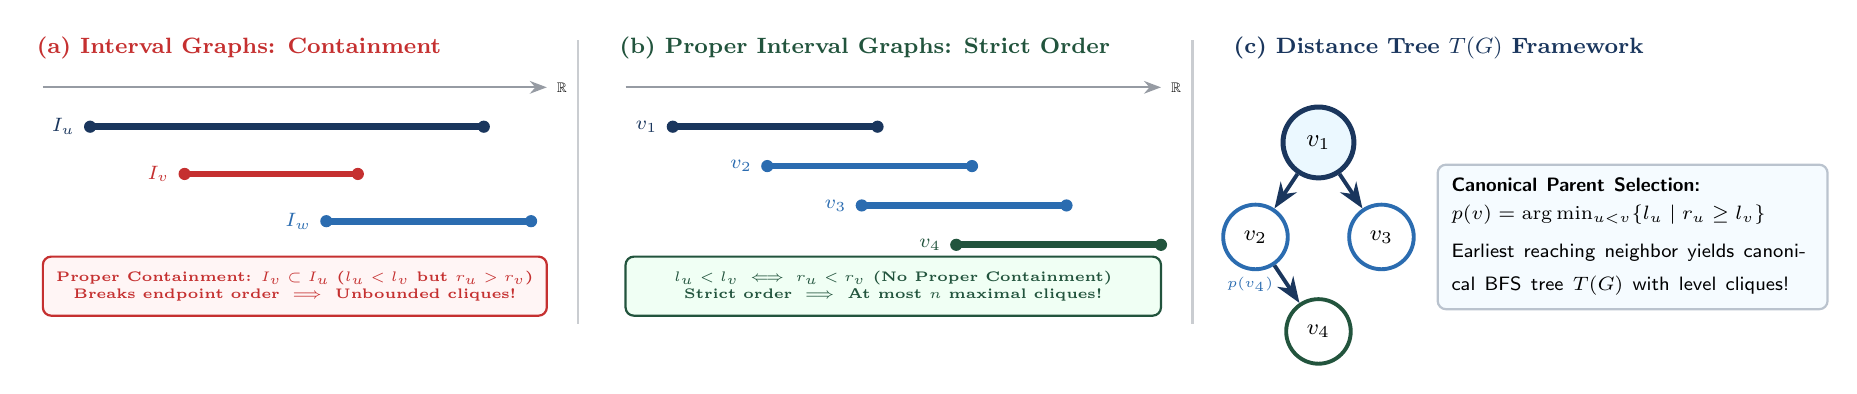
\begin{tikzpicture}[
    scale=1.0,
    >=Stealth,
    font=\sffamily,
    interval/.style={line width=2.4pt, line cap=round},
    treeNode/.style={circle, draw=navy, fill=white, line width=1.4pt, minimum size=0.82cm, inner sep=0pt, font=\bfseries\footnotesize},
    rootNode/.style={circle, draw=navy, fill=softblue, line width=1.8pt, minimum size=0.90cm, inner sep=0pt, font=\bfseries\small},
    treeEdge/.style={->, line width=1.4pt, draw=navy}
]

    % ========================================================
    % PANEL A: GENERAL INTERVAL GRAPH (Containment Allowed)
    % ========================================================
    \node[anchor=west, font=\bfseries\footnotesize, text=darkred] at (0.2, 3.4) {\textbf{(a) Interval Graphs: Containment}};
    \draw[->, line width=0.7pt, draw=darkgray!50] (0.4, 2.9) -- (6.8, 2.9) node[right, font=\tiny\bfseries] {$\mathbb{R}$};

    % Intervals with containment: u contains v properly
    \node[left=2pt, font=\scriptsize\bfseries, text=navy] at (1.0, 2.4) {$I_u$};
    \draw[interval, draw=navy] (1.0, 2.4) -- (6.0, 2.4);
    \fill[navy] (1.0, 2.4) circle (2.2pt); \fill[navy] (6.0, 2.4) circle (2.2pt);

    \node[left=2pt, font=\scriptsize\bfseries, text=darkred] at (2.2, 1.8) {$I_v$};
    \draw[interval, draw=darkred] (2.2, 1.8) -- (4.4, 1.8);
    \fill[darkred] (2.2, 1.8) circle (2.2pt); \fill[darkred] (4.4, 1.8) circle (2.2pt);

    \node[left=2pt, font=\scriptsize\bfseries, text=accentblue] at (4.0, 1.2) {$I_w$};
    \draw[interval, draw=accentblue] (4.0, 1.2) -- (6.6, 1.2);
    \fill[accentblue] (4.0, 1.2) circle (2.2pt); \fill[accentblue] (6.6, 1.2) circle (2.2pt);

    % Containment annotation badge
    \draw[draw=darkred, fill=softred, rounded corners=3pt, line width=0.8pt] 
        (0.4, 0.0) rectangle (6.8, 0.75);
    \node[font=\tiny\bfseries, text=darkred, align=center] at (3.6, 0.375) {
        Proper Containment: $I_v \subset I_u$ ($l_u < l_v$ but $r_u > r_v$)\\
        Breaks endpoint order $\implies$ Unbounded cliques!
    };

    % Divider
    \draw[line width=0.8pt, draw=darkgray!25] (7.2, -0.1) -- (7.2, 3.5);

    % ========================================================
    % PANEL B: PROPER INTERVAL GRAPH (No Containment)
    % ========================================================
    \node[anchor=west, font=\bfseries\footnotesize, text=darkgreen] at (7.6, 3.4) {\textbf{(b) Proper Interval Graphs: Strict Order}};
    \draw[->, line width=0.7pt, draw=darkgray!50] (7.8, 2.9) -- (14.6, 2.9) node[right, font=\tiny\bfseries] {$\mathbb{R}$};

    % Proper intervals: l_1 < l_2 < l_3 < l_4 <=> r_1 < r_2 < r_3 < r_4
    \node[left=2pt, font=\scriptsize\bfseries, text=navy] at (8.4, 2.4) {$v_1$};
    \draw[interval, draw=navy] (8.4, 2.4) -- (11.0, 2.4);
    \fill[navy] (8.4, 2.4) circle (2.2pt); \fill[navy] (11.0, 2.4) circle (2.2pt);

    \node[left=2pt, font=\scriptsize\bfseries, text=accentblue] at (9.6, 1.9) {$v_2$};
    \draw[interval, draw=accentblue] (9.6, 1.9) -- (12.2, 1.9);
    \fill[accentblue] (9.6, 1.9) circle (2.2pt); \fill[accentblue] (12.2, 1.9) circle (2.2pt);

    \node[left=2pt, font=\scriptsize\bfseries, text=accentblue] at (10.8, 1.4) {$v_3$};
    \draw[interval, draw=accentblue] (10.8, 1.4) -- (13.4, 1.4);
    \fill[accentblue] (10.8, 1.4) circle (2.2pt); \fill[accentblue] (13.4, 1.4) circle (2.2pt);

    \node[left=2pt, font=\scriptsize\bfseries, text=darkgreen] at (12.0, 0.9) {$v_4$};
    \draw[interval, draw=darkgreen] (12.0, 0.9) -- (14.6, 0.9);
    \fill[darkgreen] (12.0, 0.9) circle (2.2pt); \fill[darkgreen] (14.6, 0.9) circle (2.2pt);

    % Strict ordering badge
    \draw[draw=darkgreen, fill=softgreen, rounded corners=3pt, line width=0.8pt] 
        (7.8, 0.0) rectangle (14.6, 0.75);
    \node[font=\tiny\bfseries, text=darkgreen, align=center] at (11.2, 0.375) {
        $l_u < l_v \iff r_u < r_v$ (No Proper Containment)\\
        Strict order $\implies$ At most $n$ maximal cliques!
    };

    % Divider
    \draw[line width=0.8pt, draw=darkgray!25] (15.0, -0.1) -- (15.0, 3.5);

    % ========================================================
    % PANEL C: CANONICAL DISTANCE TREE CONCEPT
    % ========================================================
    \node[anchor=west, font=\bfseries\footnotesize, text=navy] at (15.4, 3.4) {\textbf{(c) Distance Tree $T(G)$ Framework}};

    % Mini tree diagram
    \node[rootNode] (t_v1) at (16.6, 2.2) {$v_1$};
    \node[treeNode, draw=accentblue] (t_v2) at (15.8, 1.0) {$v_2$};
    \node[treeNode, draw=accentblue] (t_v3) at (17.4, 1.0) {$v_3$};
    \node[treeNode, draw=darkgreen] (t_v4) at (16.6, -0.2) {$v_4$};

    \draw[treeEdge] (t_v1) -- (t_v2);
    \draw[treeEdge] (t_v1) -- (t_v3);
    \draw[treeEdge] (t_v2) -- (t_v4) node[midway, left=1pt, font=\tiny\bfseries, text=accentblue] {$p(v_4)$};

    % Rule badge on right
    \node[draw=navy!30, fill=softblue!50, rounded corners=3pt, line width=0.8pt, anchor=west, inner sep=5pt, text width=4.6cm] 
        at (18.1, 1.0) {
        \textbf{\scriptsize Canonical Parent Selection:}\\
        \vspace{1.5pt}
        \fontsize{7.2}{8.6}\selectfont
        $p(v) = \arg\min_{u < v} \{ l_u \mid r_u \ge l_v \}$\\
        \vspace{1.5pt}
        Earliest reaching neighbor yields canonical BFS tree $T(G)$ with level cliques!
    };

\end{tikzpicture}
\end{document}
